\subsection{Charakterisierung des Lasers auf der roten Linie}

\subsubsection{Aufbau}

kleiner head

\subsubsection{Aufnahme der Kennlinien}


\begin{figure}[H]
\begin{center}
  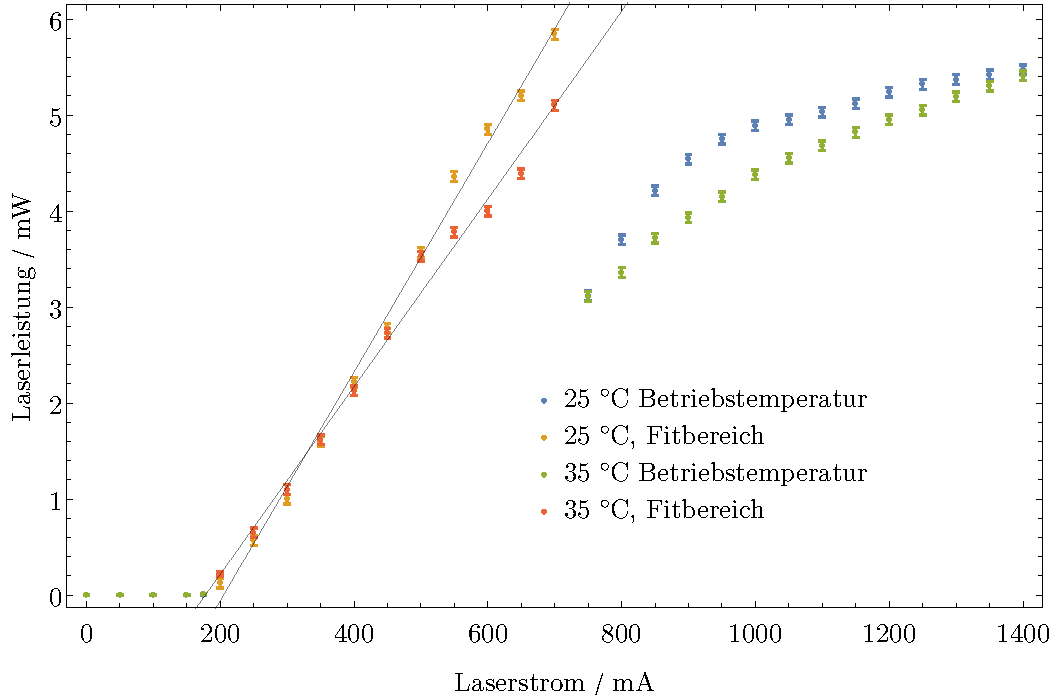
\includegraphics[width=\textwidth]{PI_rot.pdf}
  \caption{PI-Kennlinie des roten Lasers bei 25\grad und 35\grad
  Betriebstemperatur. Der modulationsfreie Bereich wurde mit $y=a(x-b)$
  gefittet, um die Laserschwelle~$b$ und die Effizienz~$a$ zu bestimmen.}
  \label{img:PI_rot}
\end{center}
\end{figure}


\begin{table}[htb]
\caption{Ergebnisse der Fits der PI-Kennlinien roten Lasers mit $y=a(x-b)$ von 200\,mA bis
700\,mA Laserstrom.}
\begin{center}
\begin{tabular}{|c|c|}
\hline
\textbf{25\grad} &  \\ \hline
$a$ & 11.91\,$\pm$\,0.10\,\textmu W\,/\,mA \\ \hline
$b$ & 204.9\,$\pm$\,2.3\,mA \\ \hline
\textchi$^2$ & 79.2873 \\ \hline
\textchi$^2$/\,DoF & 8.8097 \\ \hline
 &  \\ \hline
\textbf{35\grad} &  \\ \hline
$a$ & 9.77\,$\pm$\,0.07\,\textmu W\,/\,mA \\ \hline
$b$ & 177.7\,$\pm$\,1.9\,mA \\ \hline
\textchi$^2$ & 101.847 \\ \hline
\textchi$^2$/\,DoF & 11.3164 \\ \hline
\end{tabular}
\end{center}
\label{tab:Fits_PI_rot}
\end{table}

\FloatBarrier

\subsubsection{Messung der Laserleistung mit Photodiode}



\subsubsection{Erzeugung verschiedener Moden}


\subsubsection{Messung des dynamischen Verhaltens}

\begin{figure}[H]
\begin{center}
  \includegraphics[width=.7\textwidth]{LaserEinschwingvorgang.png}
  \caption{Photodiodenspannung (blau) nach Einschalten der Laserspannung (gelb).
  Ein dynamisches Einschwingen der Laserintensität ist erkennbar.}
  \label{img:Einschwingen}
\end{center}
\end{figure}